\chapter{Additional Figures}
\label{chapter:add-figs}

%This is the first appendix. You could put some test images or verbose data in an
%appendix, if there is too much data to fit in the actual text nicely.
%
%For now, the Aalto logo variants are shown in Figure~\ref{fig:aaltologo}.

%\begin{figure}
%\begin{center}
%\subfloat[In English]{
\includegraphics[width=.8\textwidth]{images/aalto-logo-en}}
%\subfloat[Suomeksi]{
\includegraphics[width=.8\textwidth]{images/aalto-logo-fi}}
%\subfloat[P� svenska]{
\includegraphics[width=.8\textwidth]{images/aalto-logo-se}}
%\caption{Aalto logo variants}
%\label{fig:aaltologo}
%
%\end{center}
%\end{figure}

\section{Model Selection}

\begin{figure}[H]
	\centering
	\subfloat[$\sigma_\ell=10^{-2}$]{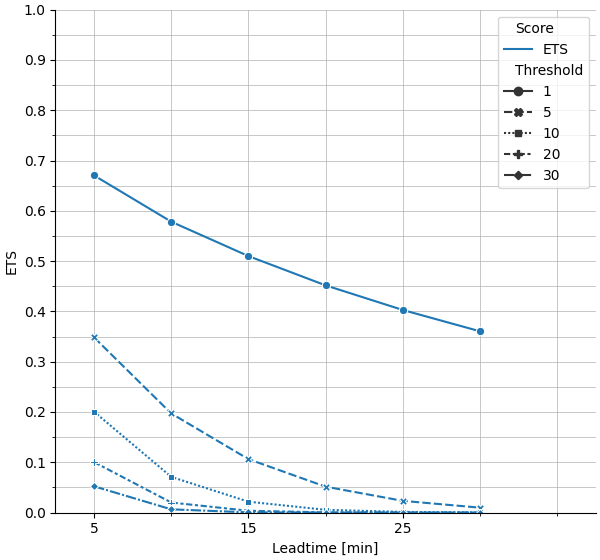
\includegraphics[width=0.45\linewidth]{images/model_choice/sigma_e-2}}
	\subfloat[$\sigma_\ell=10^{-3}$]{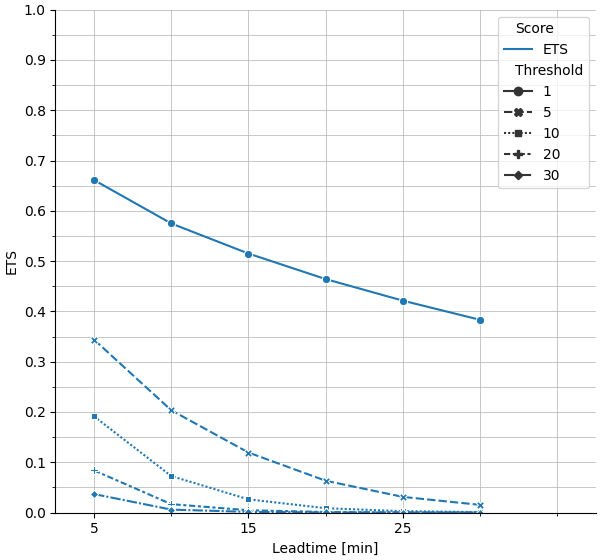
\includegraphics[width=0.45\linewidth]{images/model_choice/sigma_e-3}}
	
	\subfloat[$\sigma_\ell=10^{-4}$]{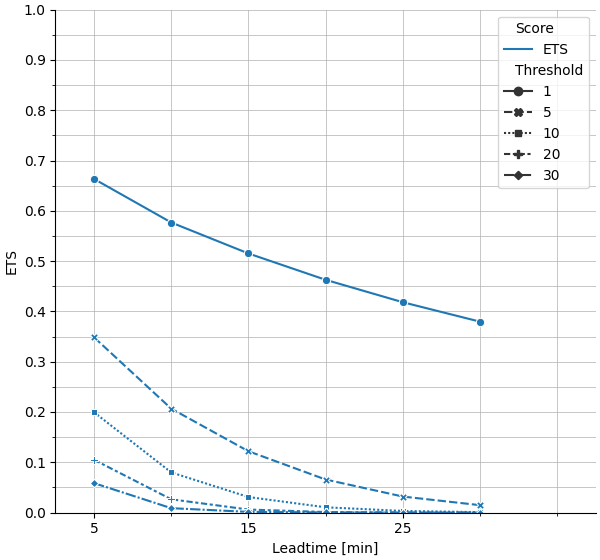
\includegraphics[width=0.45\linewidth]{images/model_choice/sigma_e-4}}
	\caption{ETS scores of RainNet over the validation set at model convergence used for choosing a $\sigma_\ell$ Gaussian NLL parameter. Thresholds are expressed in rainrate (mm/h.)}
	\label{fig:sigma_selection}
\end{figure}


\begin{figure}[H]
	\centering
	\subfloat[Equal]{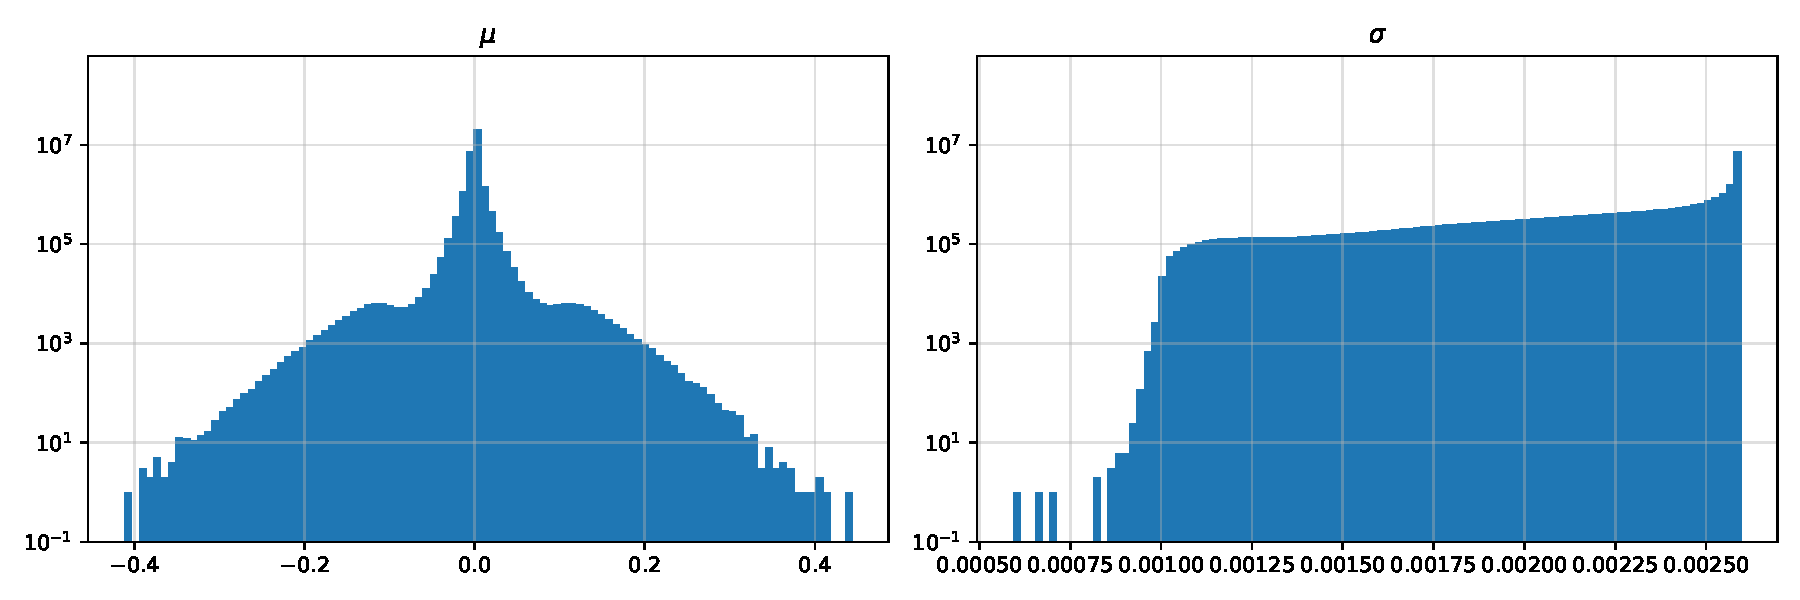
\includegraphics[width=\linewidth]{images/weight/bcnn_t2_gsm_small_diff_lt5}}
	
	\subfloat[Blundell]{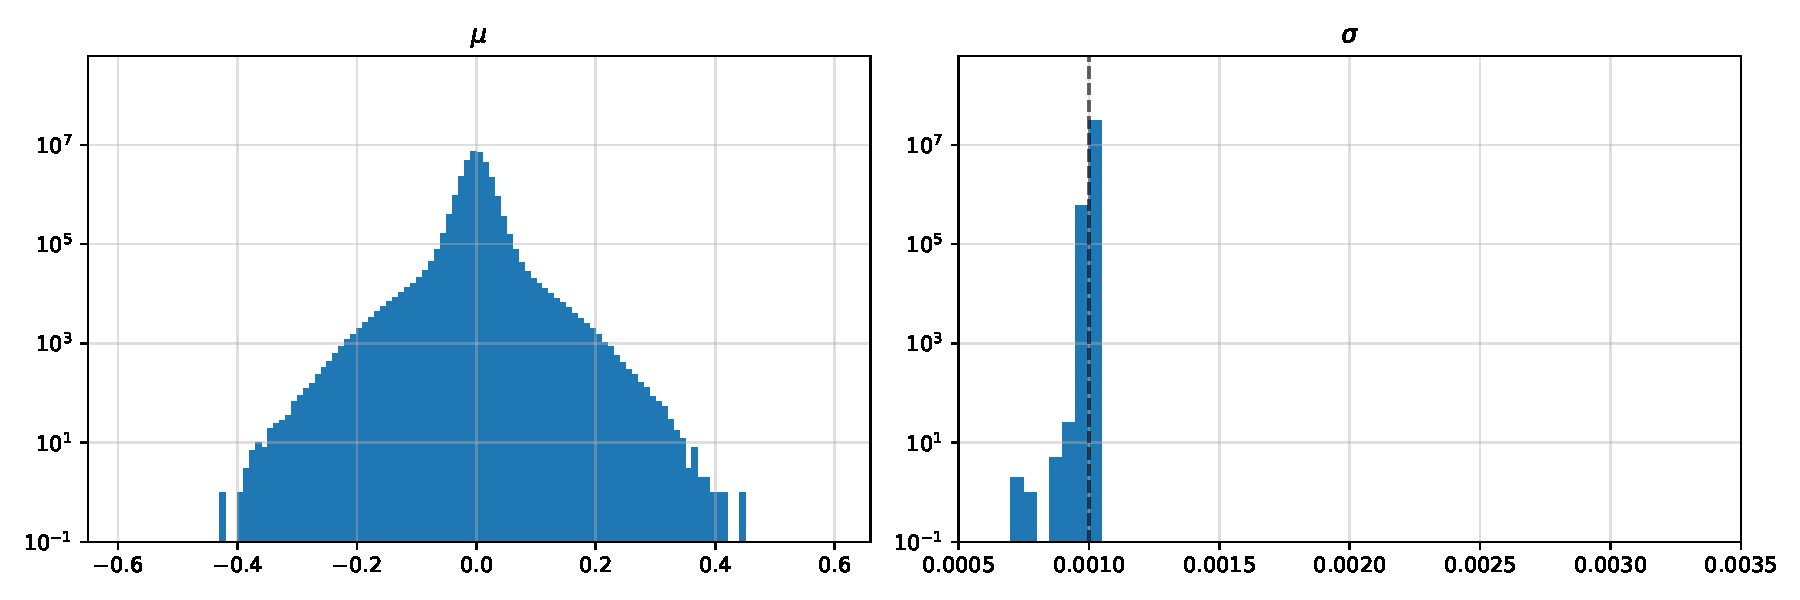
\includegraphics[width=\linewidth]{images/weight/bcnn_t2_gsm_small_diff_blundell_lt5}}
	
	\subfloat[Epoch]{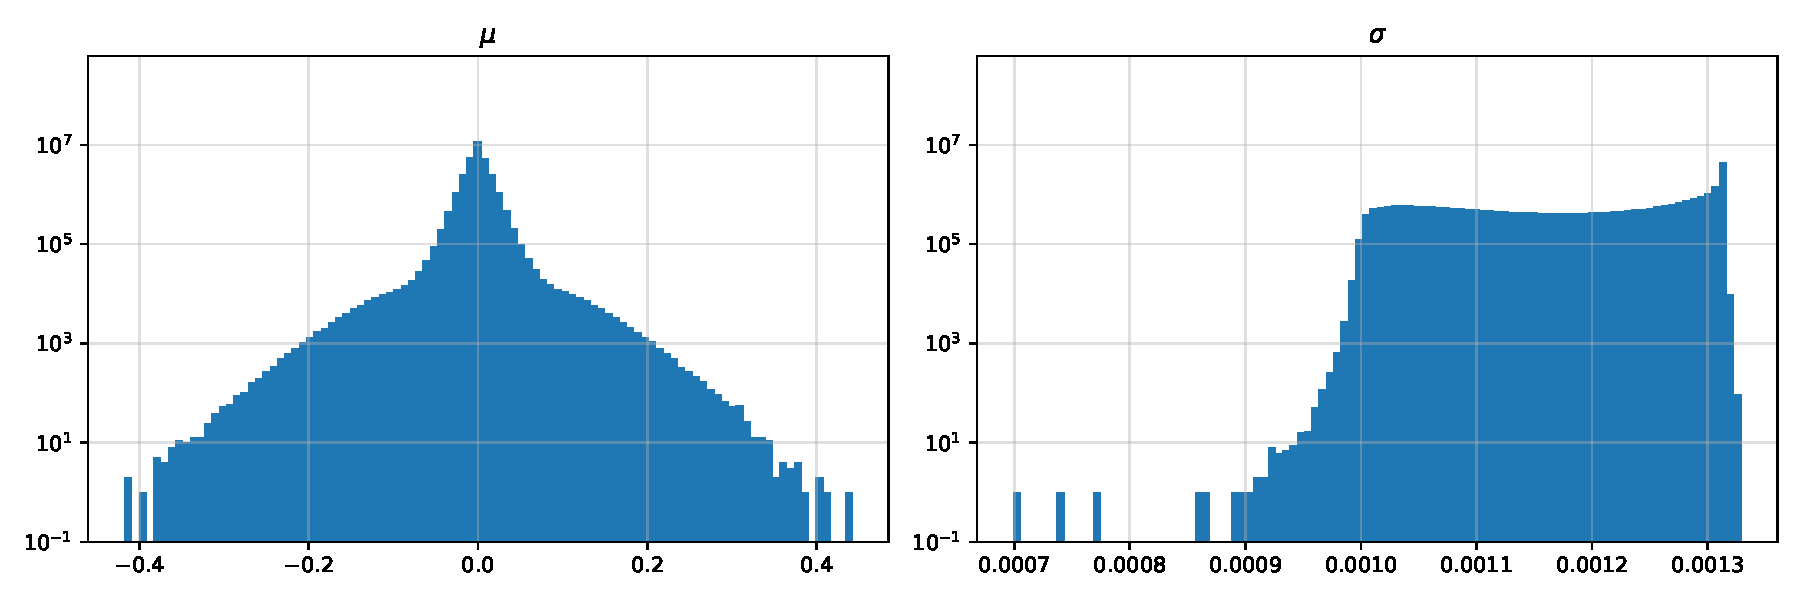
\includegraphics[width=\linewidth]{images/weight/bcnn_t2_gsm_small_diff_epoch_lt5}}
	
	\caption{The relation of complexity cost weighting scheme to the parameter posterior distributions across the network. $\mu_q$ histograms describe the parameter mean distributions, whereas $\sigma_q$ distributions describe the distribution of their standard deviations. The prior chosen is prior (4). The black dashed vertical lines indicate the initialization value for standard deviations.}
	\label{fig:bcnn-training-weights}
\end{figure}

\pagebreak

\section{Case Studies}
\label{section:additional-case-studies}

\begin{figure}[H]
	\centering
	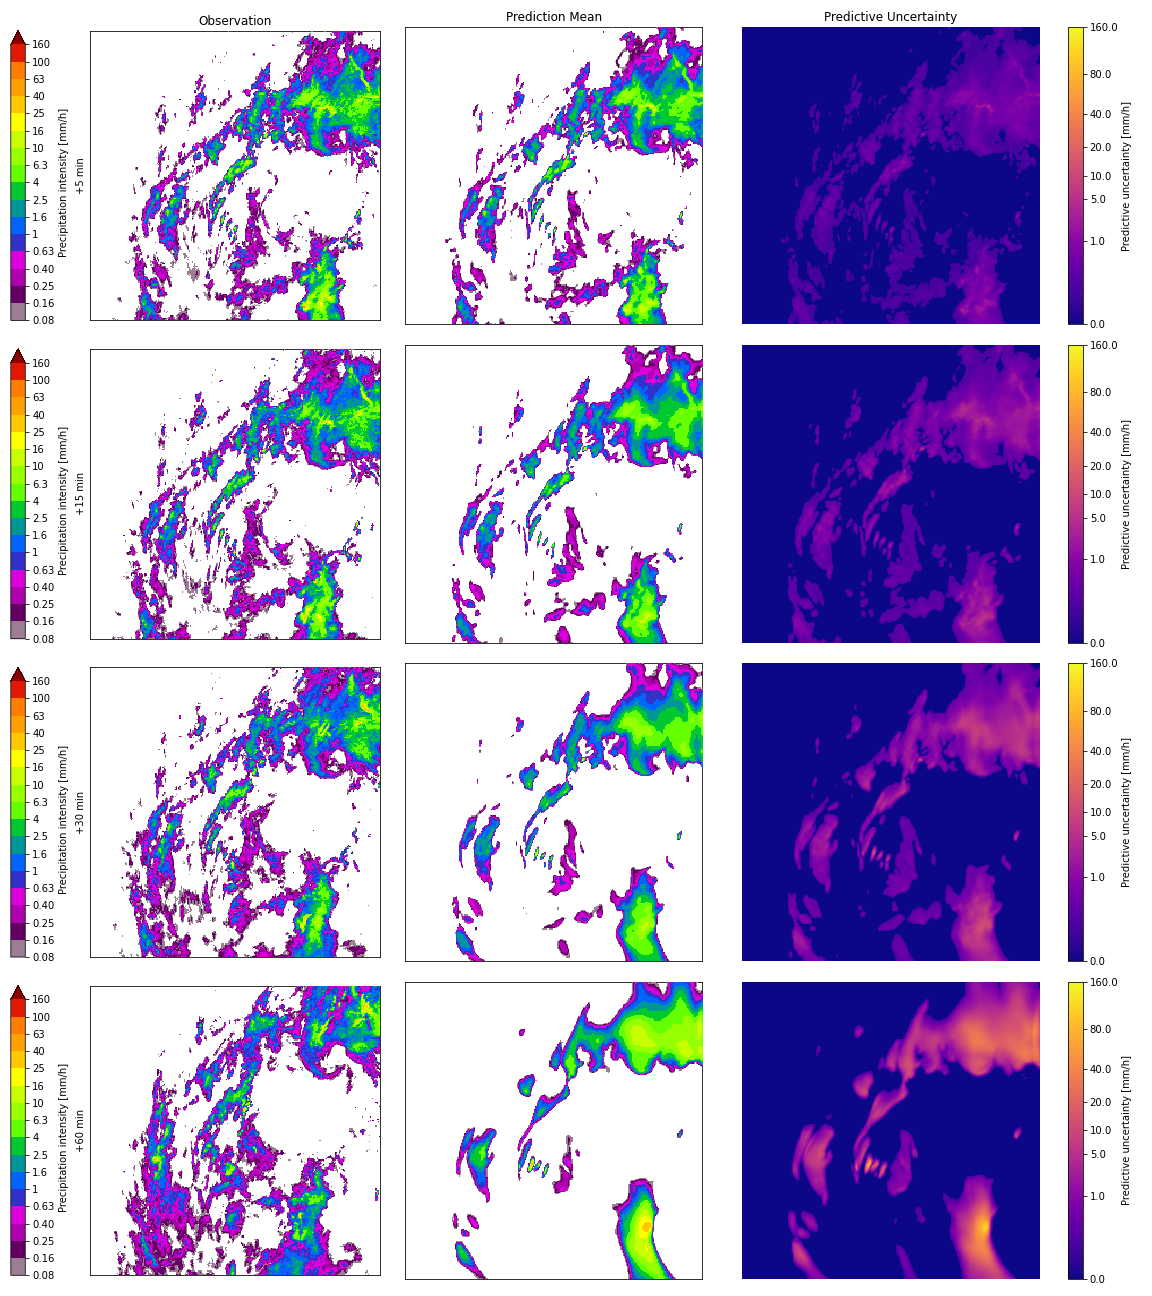
\includegraphics[width=\textwidth]{images/cases/bcnn_better_mean}
	\caption{Predictive mean and uncertainty (two standard deviations) for Case 1 on the 25th of May 2019 starting at 13:00 local Helsinki time for the \texttt{BCNN lt5 new} model, covering the area of southern Finland.}
	\label{fig:bcnn_better_mean}
\end{figure}

\begin{figure}[H]
	\centering
	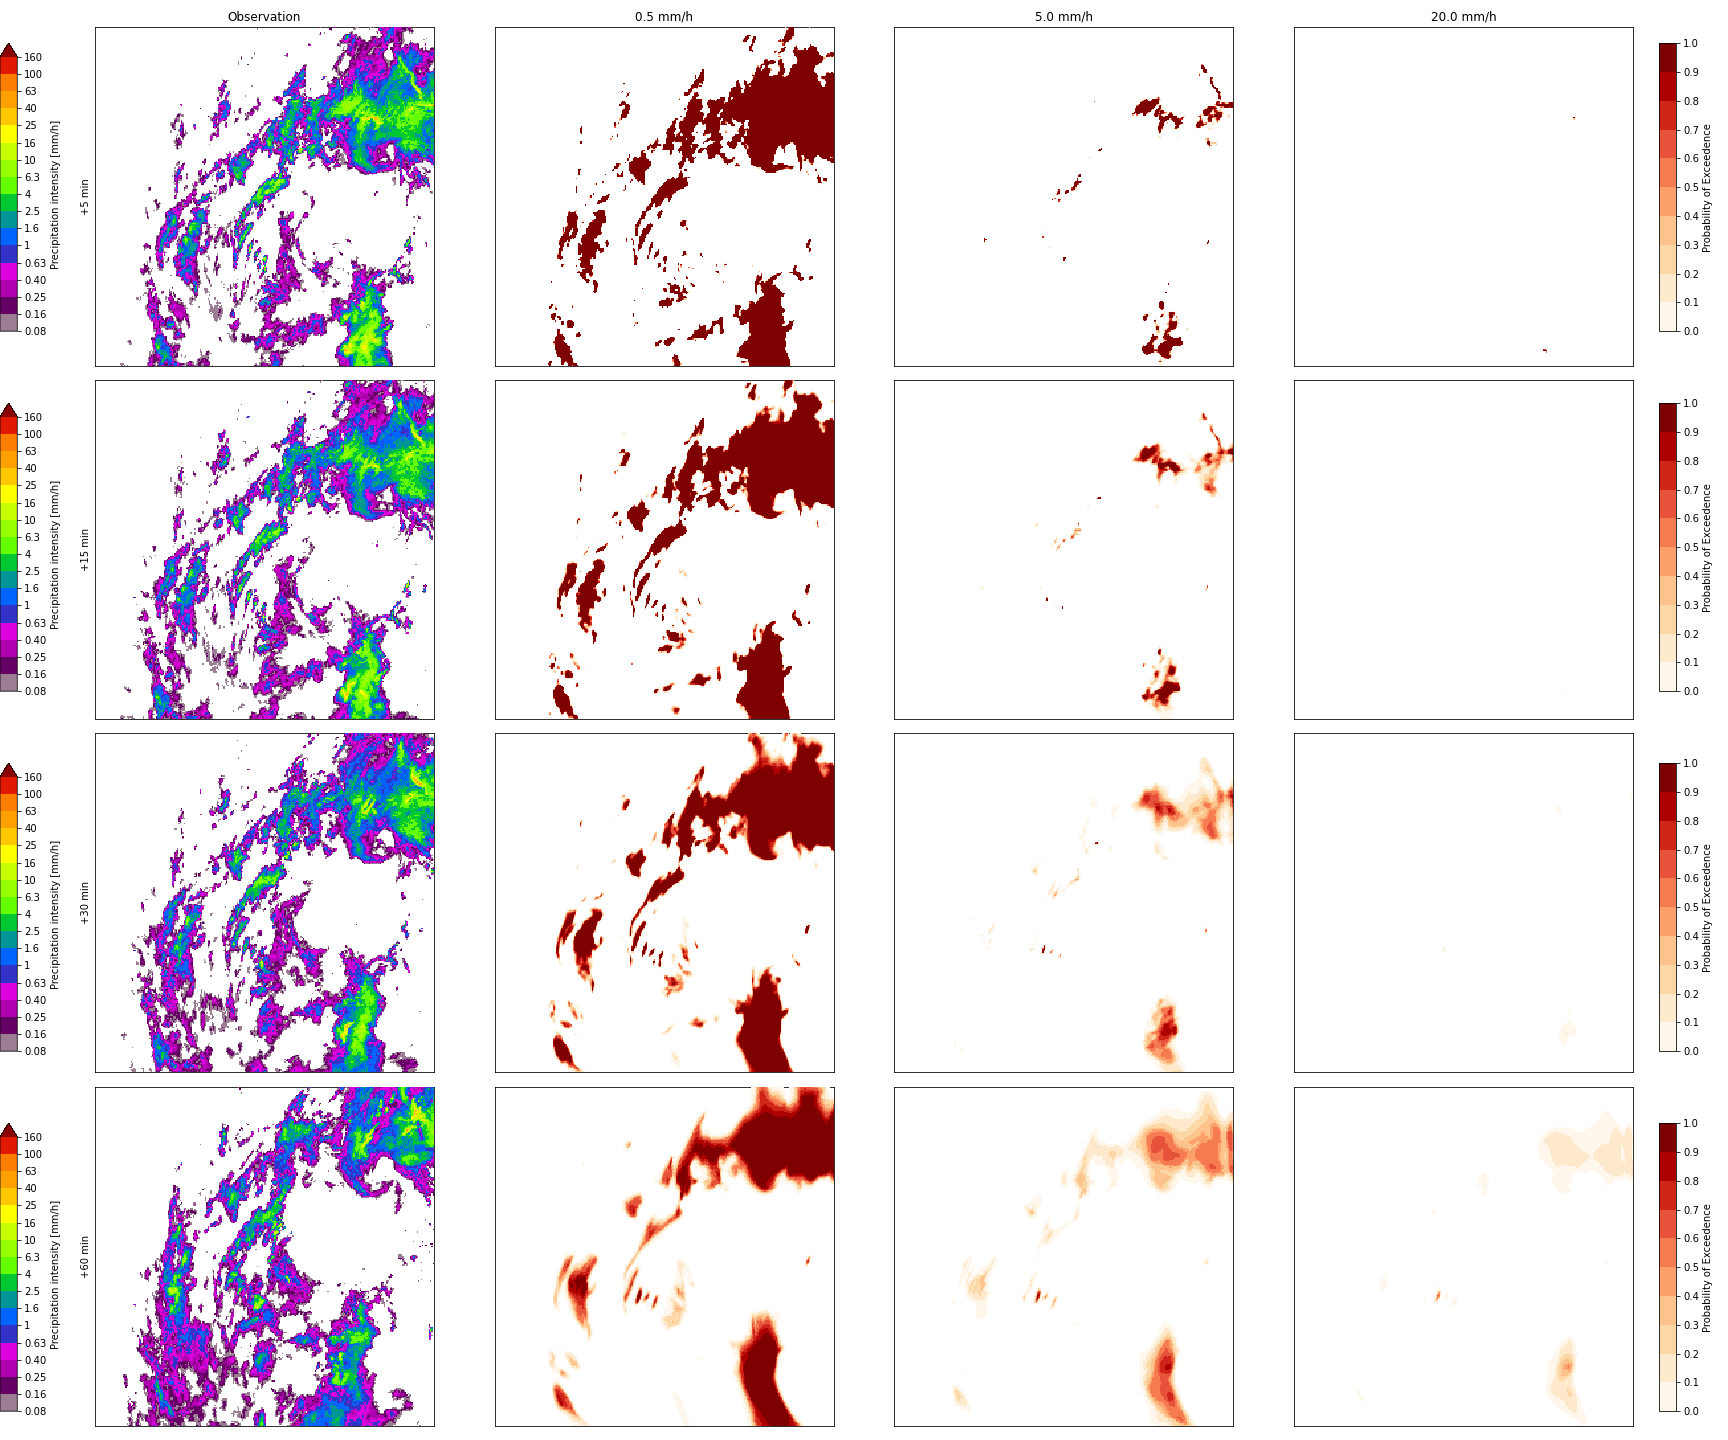
\includegraphics[width=\textwidth]{images/cases/bcnn_better_prob}
	\caption{0.5, 5.0, and 20.0 mm/h exceedance probabilities for Case 1 on the 25th of May 2019 starting at 13:00 local Helsinki time for the \texttt{BCNN lt5 new} model, covering the area of southern Finland.}
	\label{fig:bcnn_better_prob}
\end{figure}

\begin{figure}[H]
	\centering
	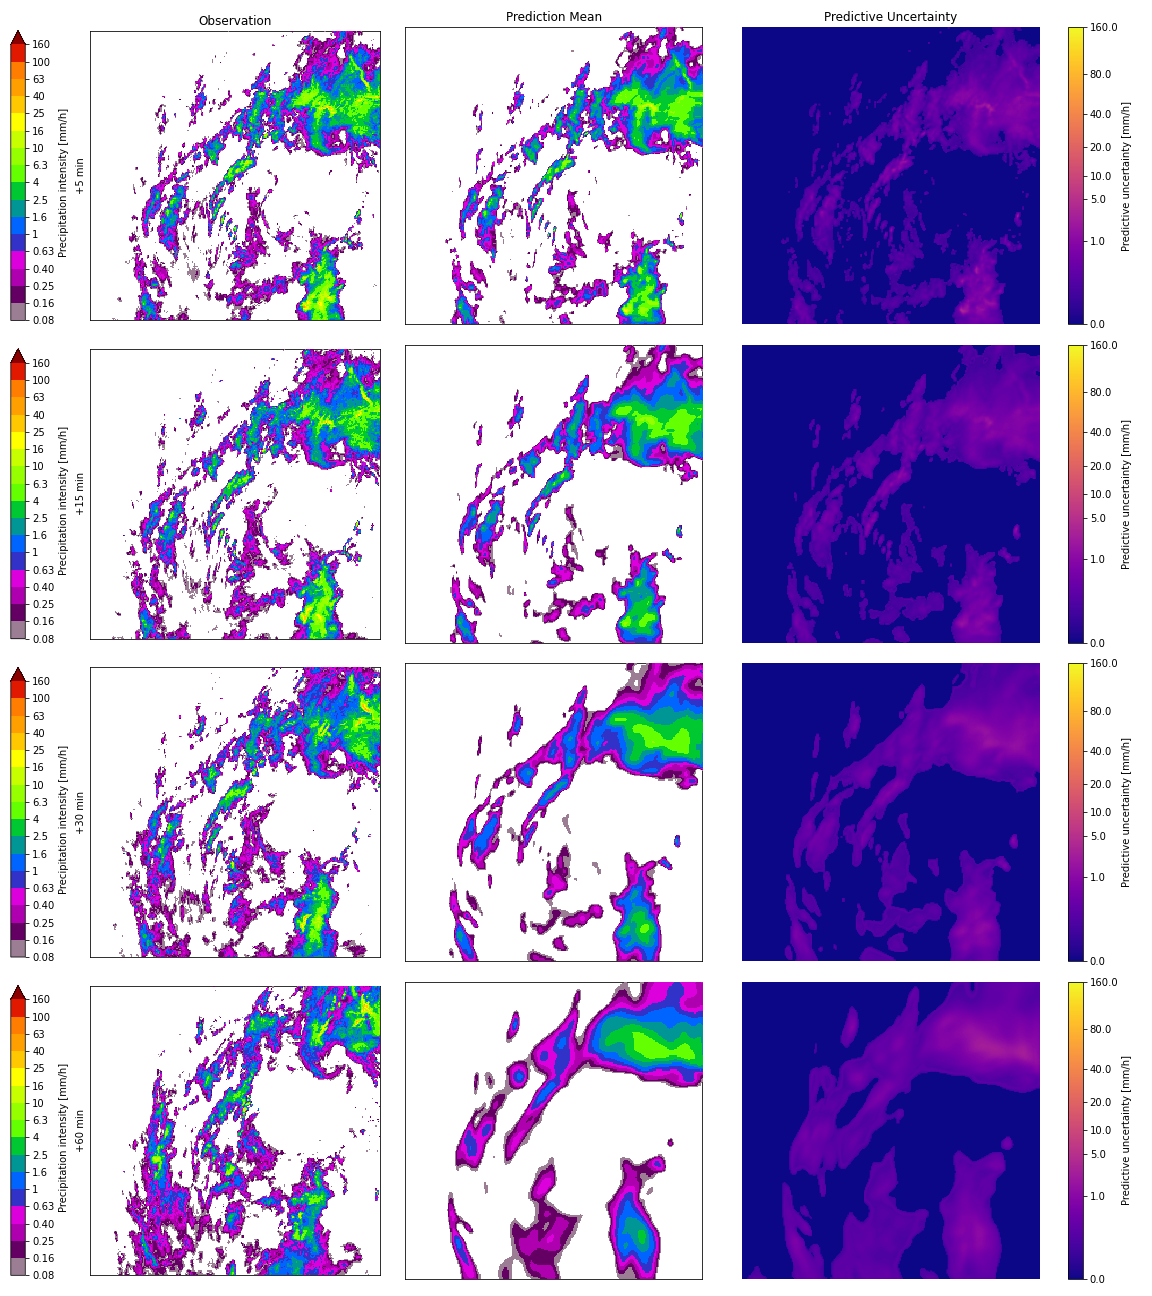
\includegraphics[width=\textwidth]{images/cases/bcnn_p2_lt30_mean}
	\caption{Predictive mean and uncertainty (two standard deviations) for Case 1 on the 25th of May 2019 starting at 13:00 local Helsinki time for the \texttt{BCNN lt30} model, covering the area of southern Finland.}
	\label{fig:bcnn_p2_lt30_mean}
\end{figure}

\begin{figure}[H]
	\centering
	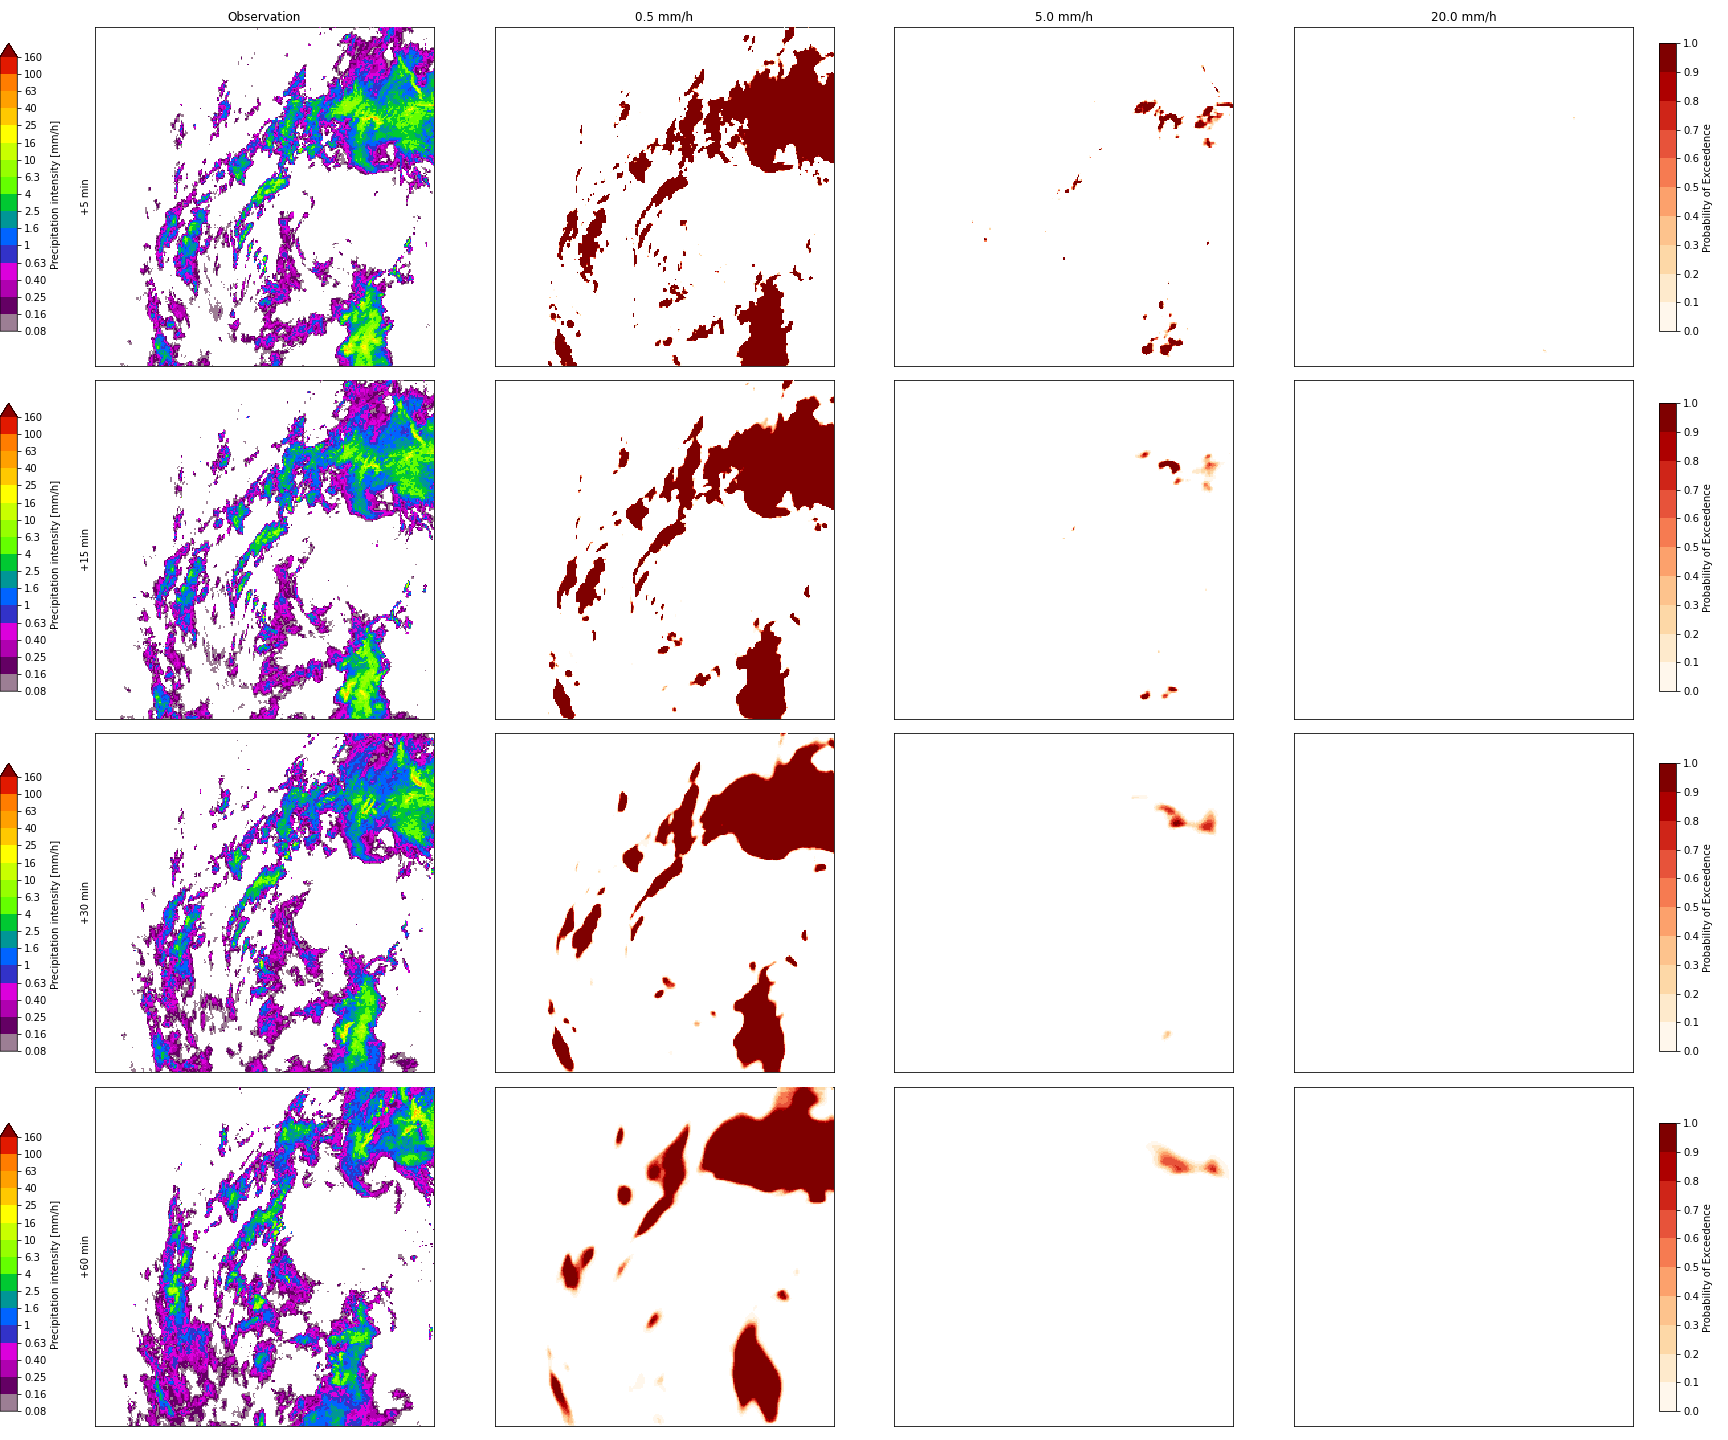
\includegraphics[width=\textwidth]{images/cases/bcnn_p2_lt30_prob}
	\caption{0.5, 5.0, and 20.0 mm/h exceedance probabilities for Case 1 on the 25th of May 2019 starting at 13:00 local Helsinki time for the \texttt{BCNN lt30} model, covering the area of southern Finland.}
	\label{fig:bcnn_p2_lt30_prob}
\end{figure}

\begin{figure}[H]
	\centering
	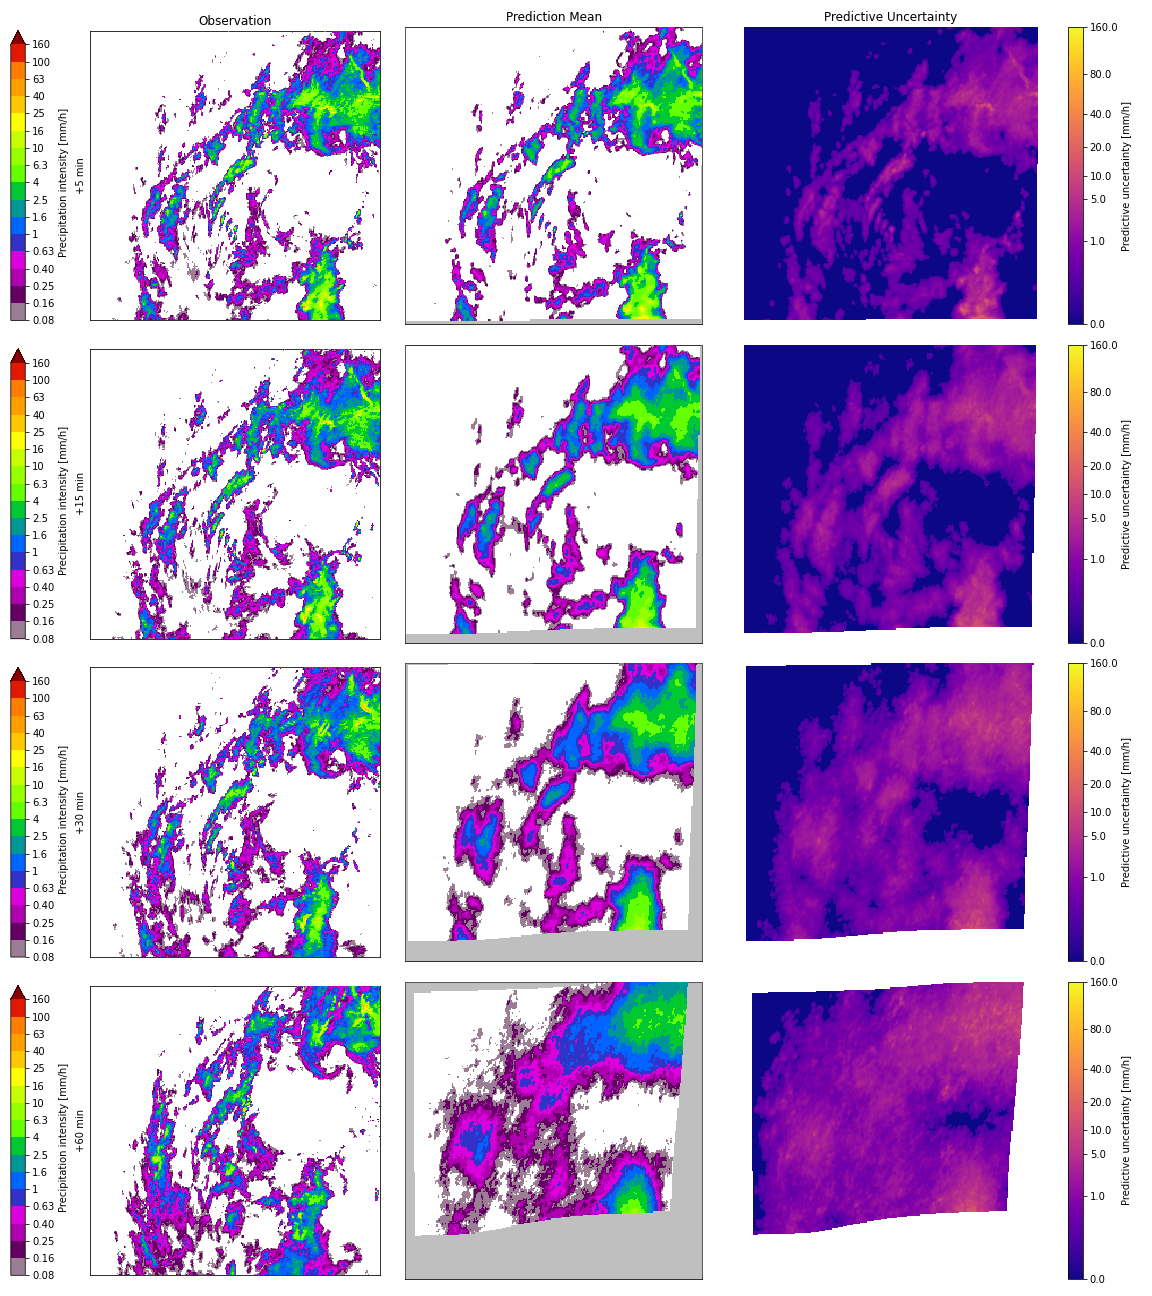
\includegraphics[width=\textwidth]{images/cases/steps_mean}
	\caption{Predictive mean and uncertainty (two standard deviations) for Case 1 on the 25th of May 2019 starting at 13:00 local Helsinki time for the baseline STEPS model, covering the area of southern Finland.}
	\label{fig:steps_mean}
\end{figure}

\begin{figure}[H]
	\centering
	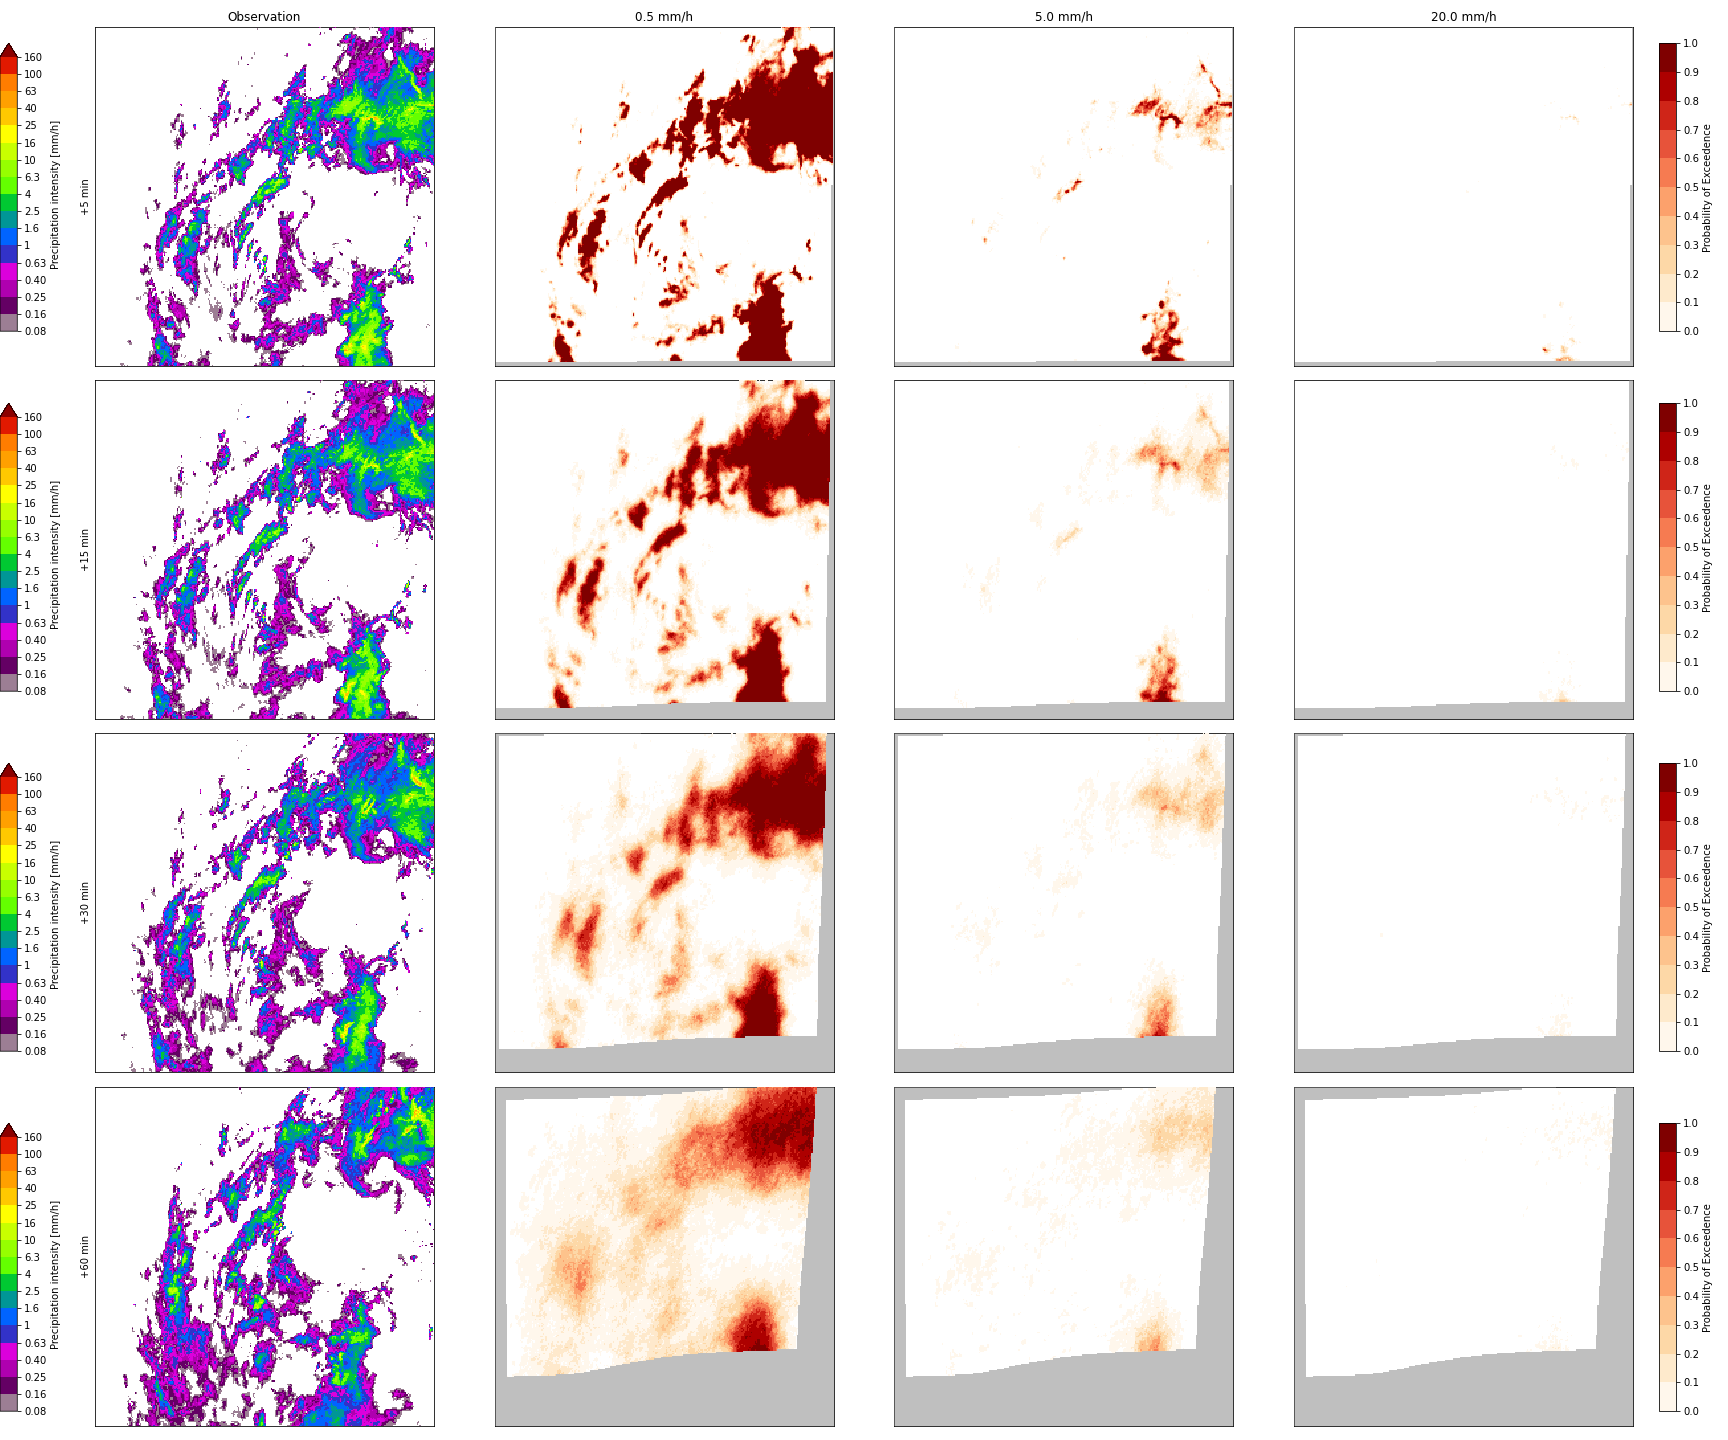
\includegraphics[width=\textwidth]{images/cases/steps_prob}
	\caption{0.5, 5.0, and 20.0 mm/h exceedance probabilities for Case 1 on the 25th of May 2019 starting at 1PM for the baseline STEPS model, covering the area of southern Finland.}
	\label{fig:steps_prob}
\end{figure}

\section{Deterministic Metrics}

\begin{figure}[H]
	\subfloat[0.5 mm/h]{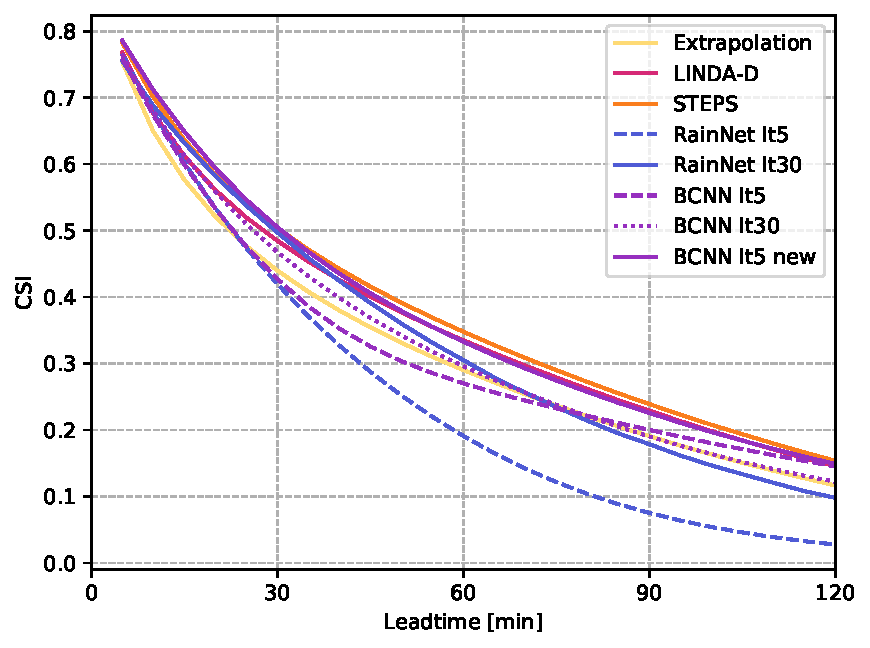
\includegraphics[width=0.33\textwidth]{images/metrics/ALL_CSI_0_5}}%
	\subfloat[5.0 mm/h]{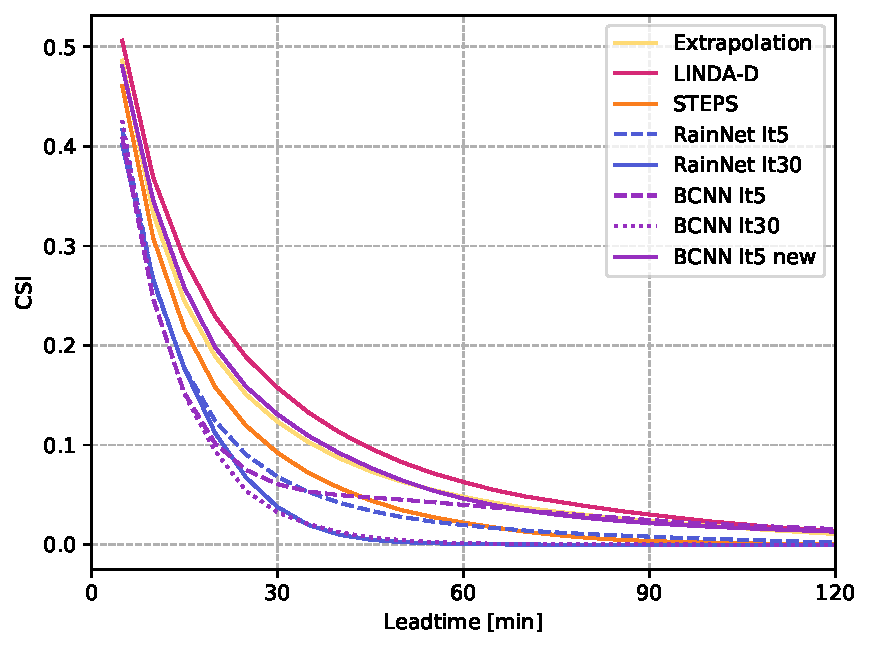
\includegraphics[width=0.33\textwidth]{images/metrics/ALL_CSI_5_0}}%
	\subfloat[20.0 mm/h]{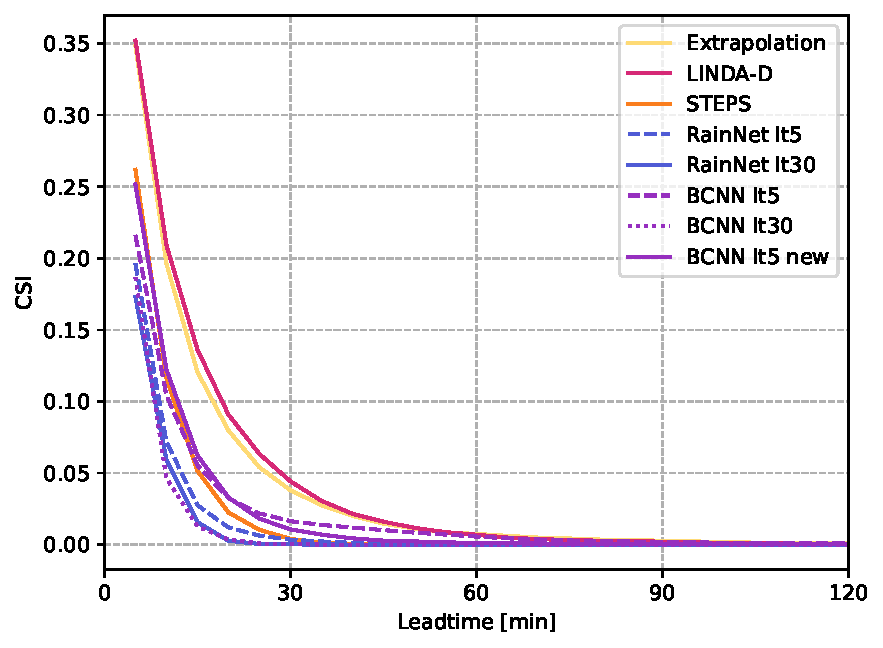
\includegraphics[width=0.33\textwidth]{images/metrics/ALL_CSI_20_0}}%
	\caption{CSI scores}
	\label{fig:csi}
\end{figure}

\begin{figure}[H]
	\subfloat[0.5 mm/h]{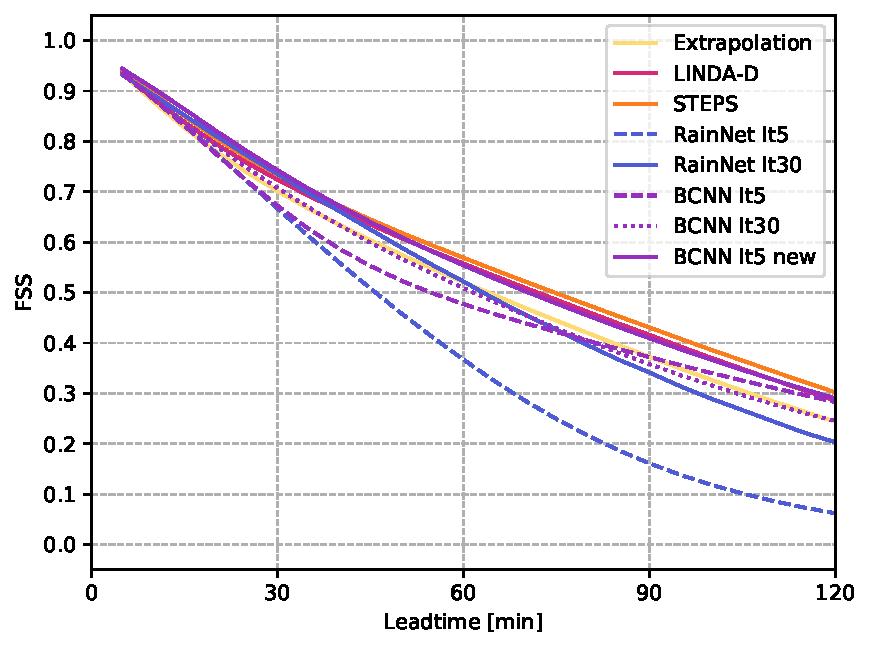
\includegraphics[width=0.33\textwidth]{images/metrics/ALL_FSS_2_0_5}}%
	\subfloat[5.0 mm/h]{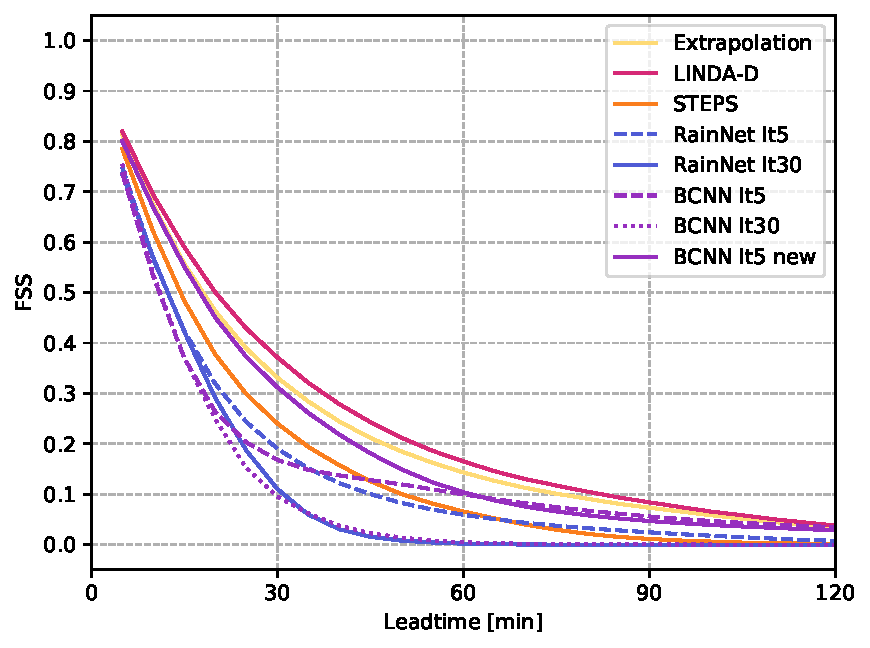
\includegraphics[width=0.33\textwidth]{images/metrics/ALL_FSS_2_5_0}}%
	\subfloat[20.0 mm/h]{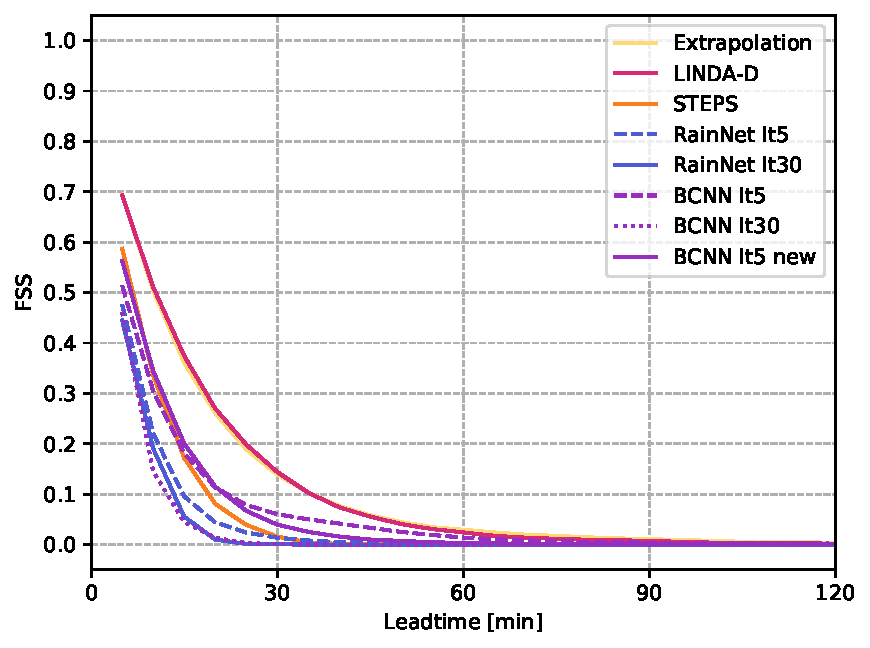
\includegraphics[width=0.33\textwidth]{images/metrics/ALL_FSS_2_20_0}}%
	\caption{FSS scores (4km)}
	\label{fig:fss4}
\end{figure}

\section{Probabilistic Metrics}


\begin{figure}[H]
	\centering
	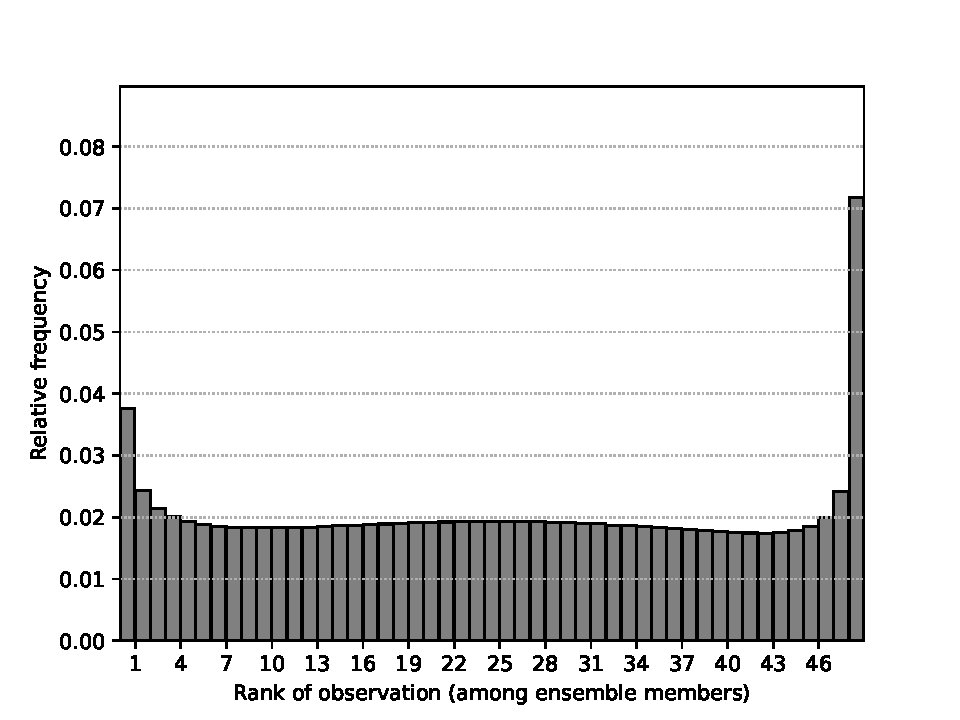
\includegraphics[width=\textwidth]{images/metrics/linda-p_rankhist_l_12}
	\caption{Rank Histogram for LINDA-P model nowcasts at a one-hour leadtime, for precipitation events exceeding 0.1 mm/h}
	\label{fig:rankhist_linda}
\end{figure}

